% Die Beamer-Klasse unterstützt folgende Optionen, die von
% besonderem Interesse sind (alle Standardoptionen werden
% ebenfalls unterstützt; siehe beamer-Basisdokumentation):
% 
%%%%%%%%%%%%%%%%%%%%%%%%%%%%%%%%%%%%%%%%%%%%%%%%%%%%%%%%%%%%%%%
% aspectratio: Seitenverhältnis des resultierenden Dokuments
% (Achtung: Aufgrund der Designvorgaben ergeben sich unterschiedliche
% Größen der effektiv nutzbaren Textblöcke)
%
% Standardeinstellung: 'aspectratio=43'
%
% Mögliche Einstellungen:
% 'aspectratio=43'   (4:3)
% 'aspectratio=169'  (16:9)
% 'aspectratio=1610' (16:10)
% 
%%%%%%%%%%%%%%%%%%%%%%%%%%%%%%%%%%%%%%%%%%%%%%%%%%%%%%%%%%%%%%%
% fontsize: Basisschriftgröße (Größen für Überschriften etc. werden
% aus dieser Basis automatisch abgeleitet)
%
% Standardeinstellung: '22pt' (entspricht den Design-Vorgaben; sehr groß!)
%
% Mögliche Einstellungen:
% '8pt', '9pt', '10pt', '11pt', '12pt', '14pt', '16pt',
% '17pt','20pt','22pt', '24pt', '26pt', '28pt'

\documentclass[aspectratio=169,16pt,xcolor=table]{beamer}

% Der OTHR-Theme unterstützt folgende Optionen:
% 
%%%%%%%%%%%%%%%%%%%%%%%%%%%%%%%%%%%%%%%%%%%%%%%%%%%%%%%%%%%%%%%
% department: (Wahl der Abteilung/Fakultät)
%
% default: 'OTHR'
%
% Mögliche Einstellungen:
% 'FakA', 'FakAM', 'FakB', 'FakBW', 'FakEI', 
% 'FakIM', 'FakM', 'FakS', 'ZWW', 'IPF',
% 'SappZ', 'KNB', 'ReMIC', 'LFD', 'LAS3',
% 'DK0PT', 'LBM', 'LeanLab', 'LFT', 'LFW',
% 'LMP', 'LMS', 'LRT', 'LWS', 'RRRU',
% 'RST', 'CEEC', 'FEM', 'IST'
%%%%%%%%%%%%%%%%%%%%%%%%%%%%%%%%%%%%%%%%%%%%%%%%%%%%%%%%%%%%%%%%%
% headerMode: Aussehen und Inhalt der Kopfleiste
%
% Standardeinstellung: 'full'
%
% Mögliche Einstellungen:
% 'full', 'frametitle', 'frametitleSection'
% 

%%%%%%%%%%%%%%%%%%%%%%%%%%%%%%%%%%%%%%%%%%%%%%%%%%%%%%%%%%%%%%%%%
% Binäre Schalter (können angegeben oder nicht angegeben werden;
% Standardeinstellung: Nicht angegeben)
%
%%%%%%%%%%%%%%%
% navbar: Navigationssymbole anzeigen (Seite vor/zurück, Kapitel vor/zurück etc.)

% pageNumbers: Seitennummerierung

% blackFont: Nur schwarze Schriftfarbe verwenden (ansonsten: Fakultätsfarben)

% frametitleCenter: Titel in der Kopfzeile zentrieren (ansonsten: rechtsbündig)

\usetheme[department=FakIM,pageNumbers]{OTHR}

% Inhaltsspezifische Zusatzpakete laden 
\usepackage[ngerman]{babel}
\usepackage[utf8]{luainputenc}
\usepackage{lipsum}
\usepackage{graphicx}
\graphicspath{ {./img/} }
\usepackage{amsmath}
\usepackage{adjustbox}
\usepackage{xcolor}
\usepackage{ulem}
\usepackage[usestackEOL]{stackengine}
\usepackage{hyperref}
\usepackage{biblatex}
\usepackage{breakcites}
\usepackage{etoolbox}


\addbibresource{ref.bib}

\patchcmd{\thebibliography}{\footnotesize}{\tiny}{}{}

% this adds the content table for each section
\AtBeginSection[]
{
  \begin{frame}
    \frametitle{Inhalt}
    \tableofcontents[currentsection]
  \end{frame}
}

\date{15. Januar 2024}

\begin{document}

\begin{frame}{YouTube Video Vorschau}
    \centering
    \href{https://www.youtube.com/watch?v=PLk8Pm_XBJE&t=612s}{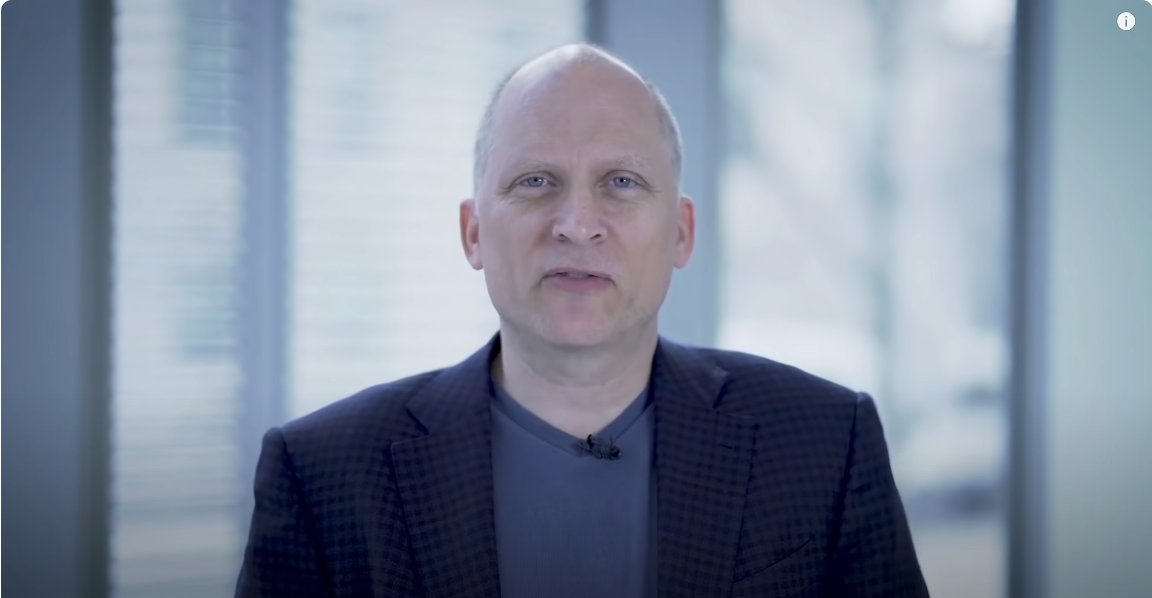
\includegraphics[width=0.8\linewidth]{pictures/Video_Vorschau.png}}
    \vspace{-0.2cm}
    \begin{flushleft}
        \tiny Quelle: \url{https://www.youtube.com/watch?v=PLk8Pm_XBJE}, zuletzt besucht am 12.12.2023
    \end{flushleft}
\end{frame}

\title{Transhumanismus}
\subtitle{Fortschritt oder Dystopie?}
\author{Marcel Ott, Nicolas Zander, Lorenz Branner, Severin Bittl, Thomas Gailinger}
\institute{Ethik in der Informatik}

\maketitle

%\begin{frame}
%	\frametitle{Inhaltsverzeichnis}
%	\tableofcontents
%\end{frame}

\section{Recap}
\subsection{Nachfrageprognose}
\begin{frame}
	\frametitle{Basics}
	\begin{itemize}
	\item Nachfrage unterliegt einer nat\"urlichen \textbf{Schwankung} und Trends~\cite{aguayo2023inklusion}
	\begin{itemize}
	\item (Saisonale Schwankung, steigende Nachfrage, nat\"urliche Varianz)
	\end{itemize}
	\item Ziel der Prognose ist es, langfristige und mittelfristige Ver\"anderungen der Nachfrage \textbf{vorhersagen} zu k\"onnen
	\item Mithilfe der Prognose wird in der operativen Planung ein \textbf{Produktionsplan} erstellt
	\end{itemize}
\end{frame}

\newpage
\printbibliography % Druckt das Literaturverzeichnis in kleinerer Schriftgröße aus

\end{document}
